\documentclass{article}

\usepackage{lastpage} % for the number of the last page in the document
\usepackage{fancyhdr}
\usepackage{geometry}
\usepackage{graphicx}
\usepackage{grffile}
\usepackage[utf8x]{inputenc}
\geometry{a4paper}
\geometry{portrait}
\pagestyle{fancy}
\usepackage{float}
\fancyhf{}
\lhead{User Manual KinderFinder}
\rhead{Section \thesection}
\lfoot{}
\rfoot{Page \thepage\ of \pageref{LastPage}}


%\begin{figure}[H]
%\centering
%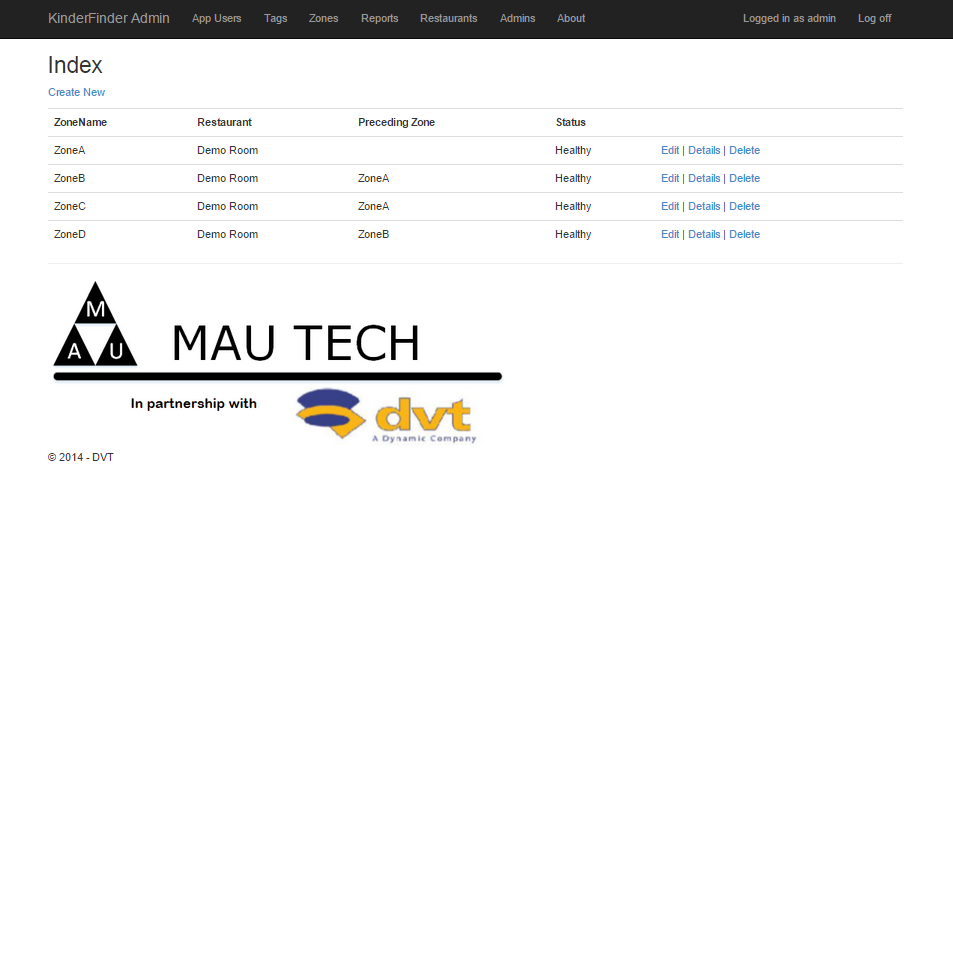
\includegraphics[scale=0.5]{adminportalzones.png}
%\caption{Use case of Android app user (first level granularity).}
%\end{figure}

\newcommand{\horrule}[1]{\rule{\linewidth}{#1}}

\title{
		\normalfont \normalsize \textsc{Client Name: DVT} \\
		\normalfont \normalsize \textsc{Project Name: KinderFinder} \\ [25pt]
		\horrule{0.5pt} \\[0.4cm]
		\huge KinderFinder User Manual \\
		\horrule{2pt} \\[0.5cm]
}
\author{\begin{tabular}{rl}
	\texttt{Team Name:} & \texttt{MAU Technologies} \\[0.5cm]
	Uteshlen Nadesan & 28163304 \\
	Michael Johnston & 12053300 \\
	Po-Han Chiu & 11063612
\end{tabular}
	\\ \\ \texttt{}
	\\ \\ \texttt{Version: 1}}
\date{20 October 2014} 


\begin{document}
\maketitle
\newpage

\tableofcontents
\newpage


\section{Welcome to KinderFinder}
\subsection{What is KinderFinder}
\paragraph{}
KinderFinder is a  solution that uses indoor tracking of people ,  to assist with a common 
problem  in  public  places.  Many  restaurants  aim  to  give  parents  a  worry  free  dining 
experience,  by providing facilities to entertain,  and safely look after their children.
\paragraph{} However, 
a parent still has the worry, and consistent need  to  ensure their children are still in the safe 
and designated areas.  KinderFinder attempts to assist the parents in being able to make 
sure their children are still in these areas without the need to get up from their tables.


\newpage
\section{About this manual}

\begin{itemize}
\item Please read this manual before using the device to ensure safe and proper use.
\item  	Please read this manual before using the device to ensure safe and proper use.
\item	Descriptions are based on the devices default settings.
\item 	Images and screen shots may differ in appearance from the actual product.
\item 	Content may differ from the final product, or from software provided by service providers 
or carriers, and is subject to change without prior notice.
\item	Content (high quality content) that requires high CPU and RAM usage will affect the 
overall performance of the device. Applications related to the content may not work 
properly depending on the devices specifications and the environment that it is used in.
\item	Available features and additional services may vary by device, software, or service 
provider.

\end{itemize}

\newpage

\section{Getting started}
\subsection{Set up}
Congratulations on your purchase of the KinderFinder system, this manual should help you get the most out of the KinderFinder system installed.

\subsection{Installation}
\subsubsection{Software}
If you are purchasing the KinderFinder software for an establishment, good news, there is minimal installation required.
All software necessary is on the cloud. Navigate on a web browser to www.kinderFinder.co.za to view the Administration Portal that will provide one with the nessessary admin tasks that will be discussed later.

\subsubsection{Room Maps}
As you are aware, KinderFinder uses a map of the room being monitored to view the locations of tags worn by users. In this regard, a map of the room must be made and uploaded to the admin portal. The .JPG format for the map file would be sufficient. On the mobile application it would look similar to figure 1 below.

\begin{figure}[H]
\centering
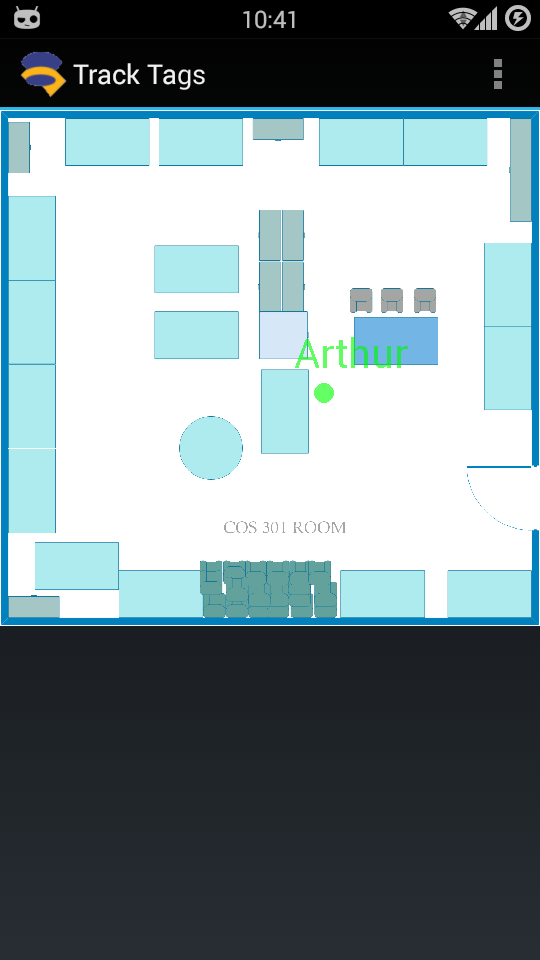
\includegraphics[scale=0.3]{MainAppTrack Tags.png}
\caption{Map view in mobile application}
\end{figure}

\subsubsection{Receivers}
Receivers are devices that pick up the signals from tags worn by users. These receivers should be placed at the edges of the room for maximum range and location capabilities.  Refer to figure 2 for the optimal places to place the receivers.

\begin{figure}[H]
\centering
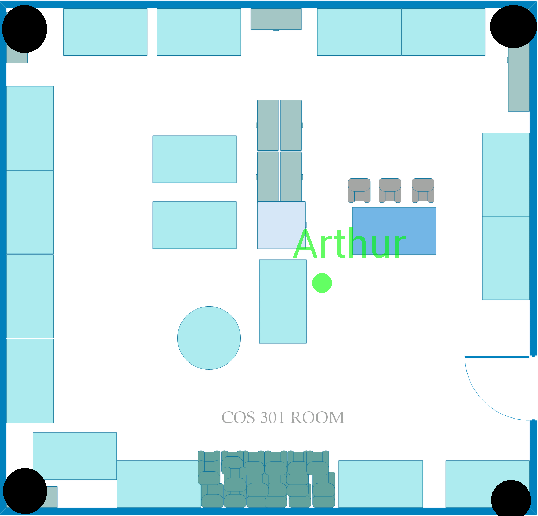
\includegraphics[scale=0.6]{pic1.png}
\caption{Optimal receiver placement}
\end{figure}

\subparagraph{Setting up Receivers}
Receivers used in KinderFinder are android mobile devices. The application that needs to be installed on these devices is called "Transmitter" and should be run from the device. Upon opening the transmitter application, choose the establishment the device will be used in and then the place in the room the device will be in X and Y Cartesian co-ordinates. Tap the "Transmit" button and the application will start to transmit to the server. Do this for all mobile devices used as receivers. 


\newpage

\section{The Administration Portal}

Each establishment will have an administrator. The job of the administrator is to add and register users, in this case, register parents who would like to know the location of their children and the assignment of tags to the users.

\subsection{Administration Portal}
The main page of the administration portal is depicted below in figure 3

\begin{figure}[H]
\centering
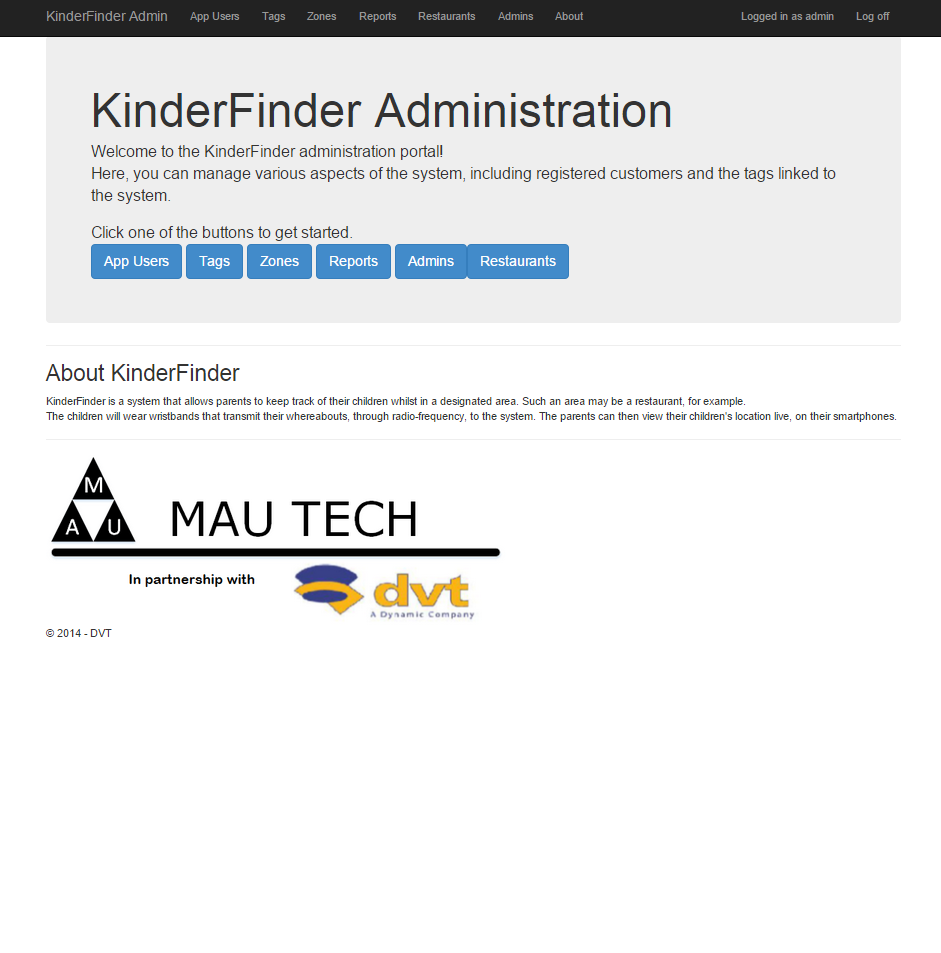
\includegraphics[scale=0.6]{adminportal2.png}
\caption{Administration Portal}
\end{figure}

\subsection{App Users}
Figure 4 below depicts the administration portal. For your establishment, all users will be shown here and can be edited and removed from the program by the admin.

\begin{figure}[H]
\centering
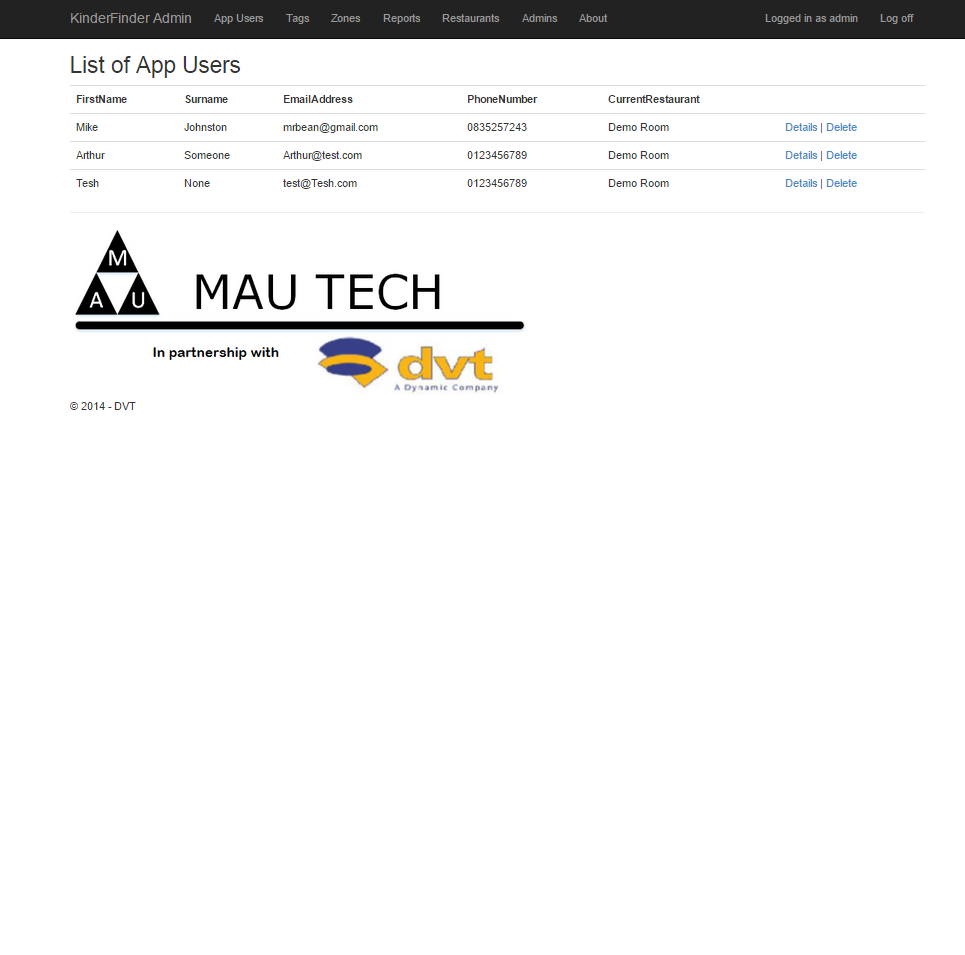
\includegraphics[scale=0.6]{adminportal3.png}
\caption{Administration Portal}
\end{figure}

\subsection{Tags}
Figure 5 below depicts the "Tags" tab. Here, admins can assign tags to registered users and either free tags or edit the usage of these tags. Also, these tags can be deemed out of order if a report shows that the tag itself no longer functions.
\begin{figure}[H]
\centering
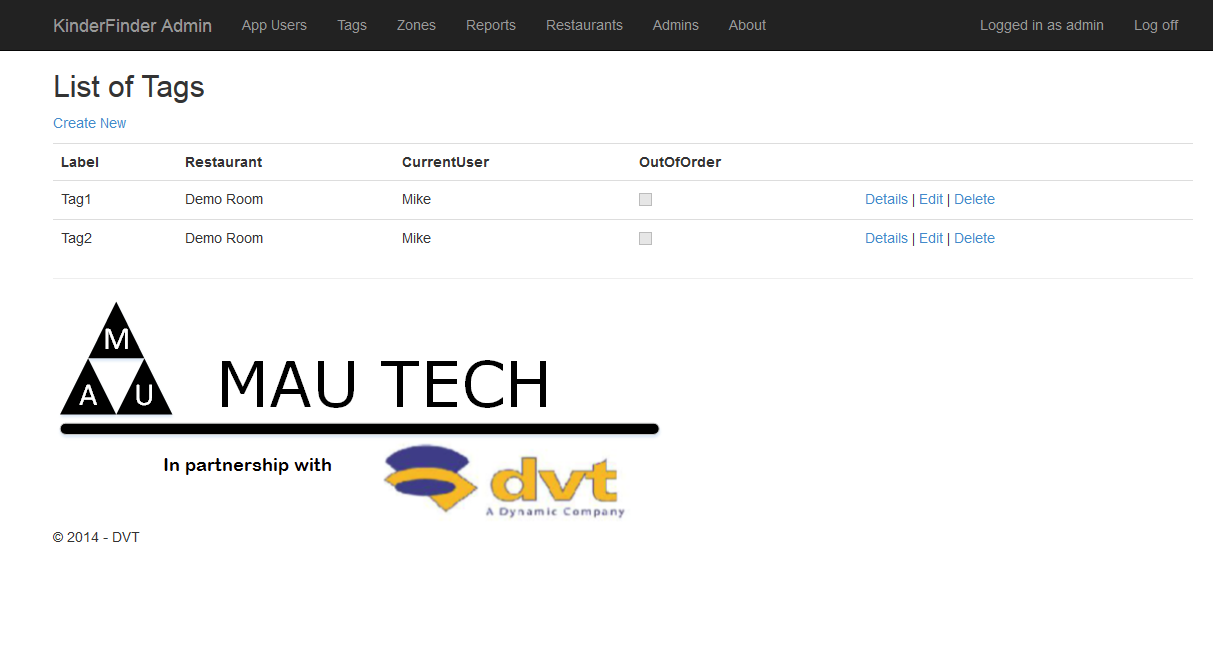
\includegraphics[scale=0.4]{tags.png}
\caption{Administration Portal}
\end{figure}

\subsection{Zones}
Each establishment will have allocated zones, places that will be monitored. Here the user can monitor zones for a particular establishment.
\begin{figure}[H]
\centering
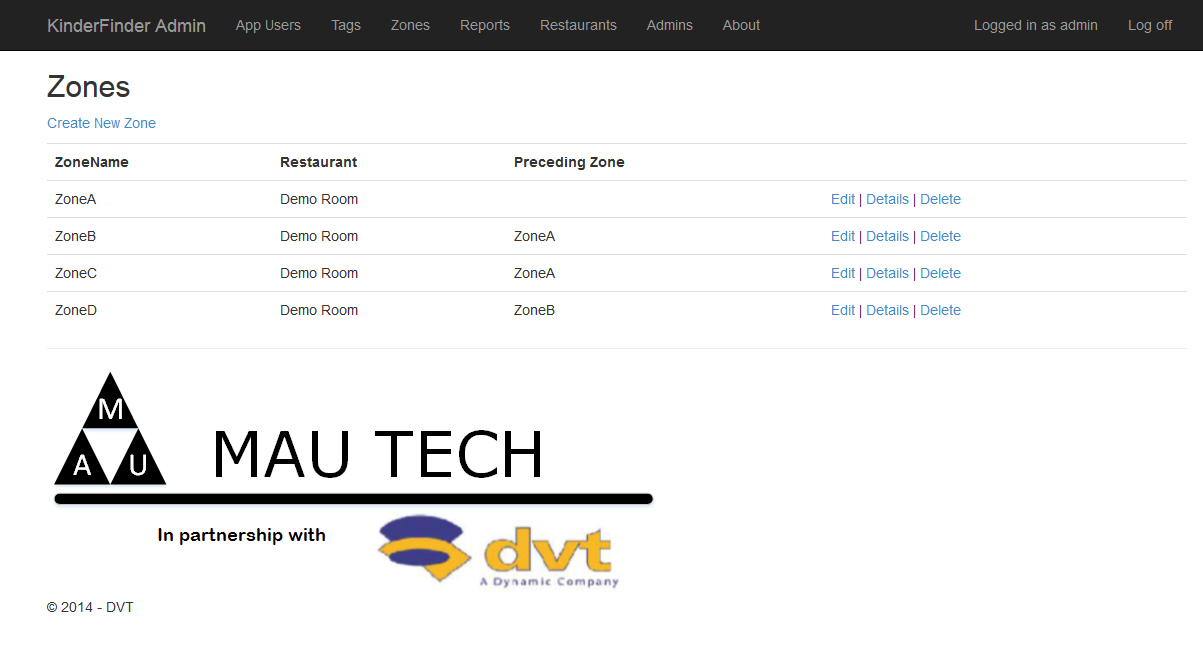
\includegraphics[scale=0.4]{zones.png}
\caption{Administration Portal}
\end{figure}

\subsection{Reports}
The reports page can generate reports for the user based on tags, zones and application users. Greater administration privileges will be needed to access some of the reports.
\begin{figure}[H]
\centering
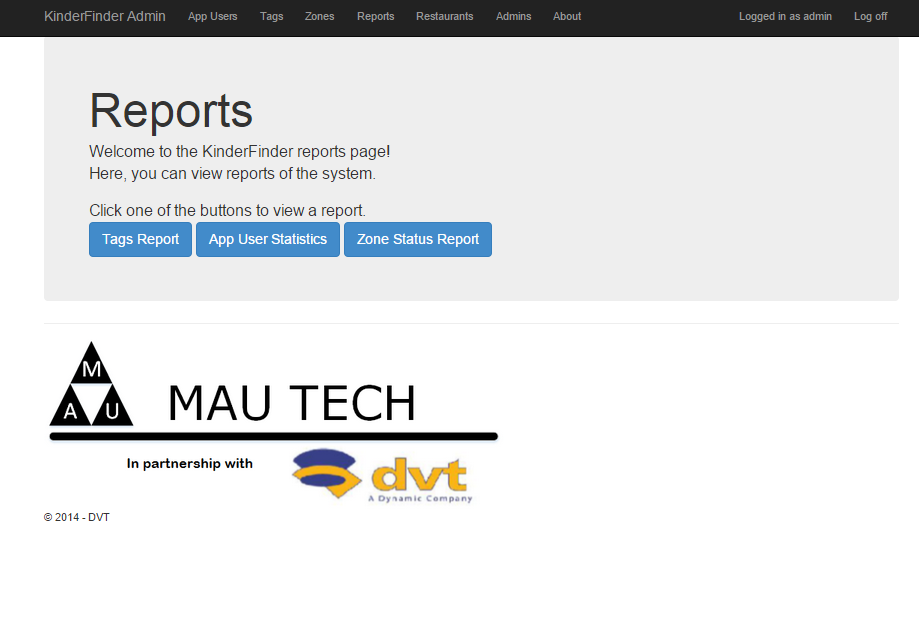
\includegraphics[scale=0.4]{adminportalreports.png}
\caption{Administration Portal}
\end{figure}

\subsection{Admins}
Here users who have higher administration privileges can add administrators to a specific establishment.
\begin{figure}[H]
\centering
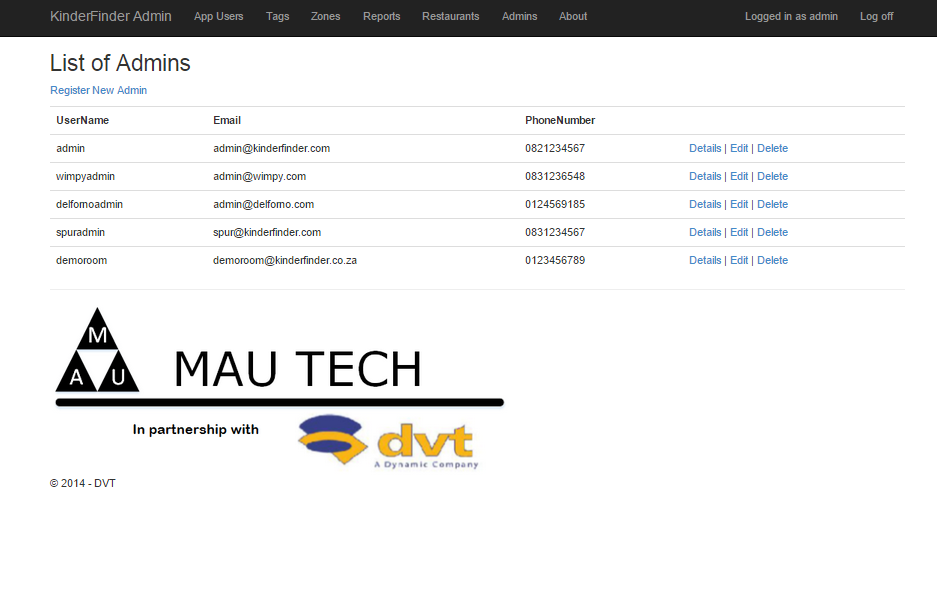
\includegraphics[scale=0.4]{adminportal3listofadmins.png}
\caption{Administration Portal}
\end{figure}

\subsection{Restaurants}
Clicking on the restaurants tab will open the list of restaurants that can be viewed, restaurants can be added and removed or edited by the system administrator.
\begin{figure}[H]
\centering
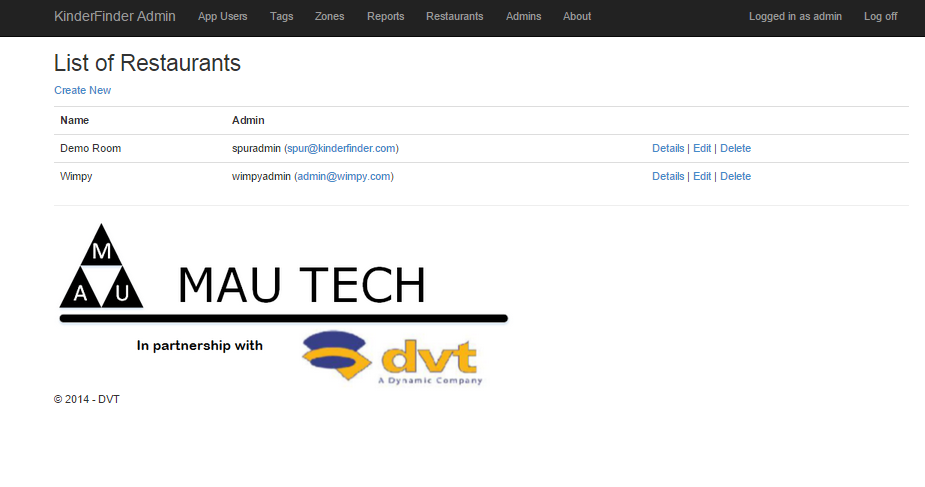
\includegraphics[scale=0.4]{adminportallistofrestaurants.png}
\caption{Administration Portal}
\end{figure}

\newpage
\section{Mobile Application - Android}
KinderFinder's main interface with its registered users is the mobile application, here one can view the locations of all the linked tags and add specific names to each tag linked to  a user's account.

\subsection{Log in}
When the app opens, this page is the first page the user will be directed to, here one can log in, or, if one has not registered with the app, click on the "register" button to register.
\begin{figure}[H]
\centering
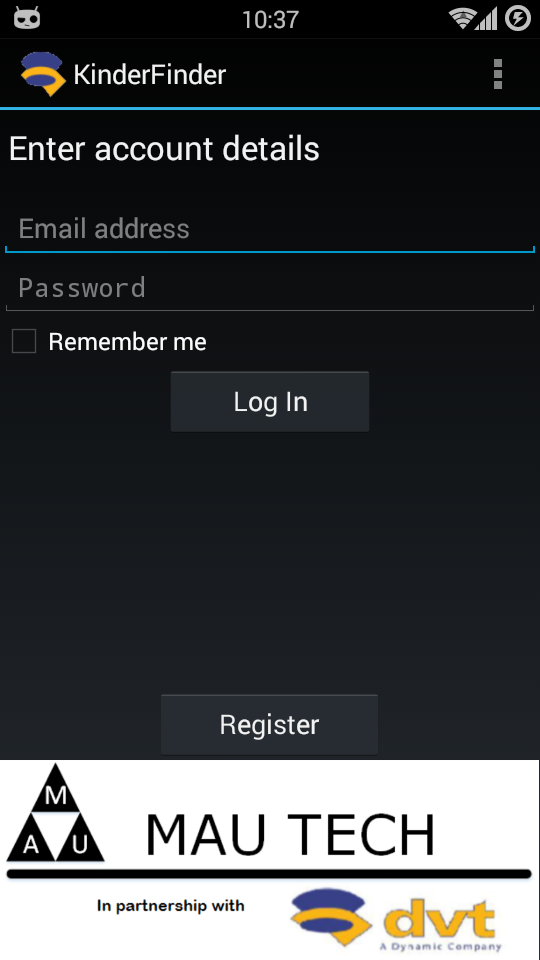
\includegraphics[scale=0.4]{Main App - Log In.png}
\caption{KinderFinder Mobile Application}
\end{figure}

\subsubsection{Registration}
To register with the application, just add your details as below in figure 11 to register.
\begin{figure}[H]
\centering
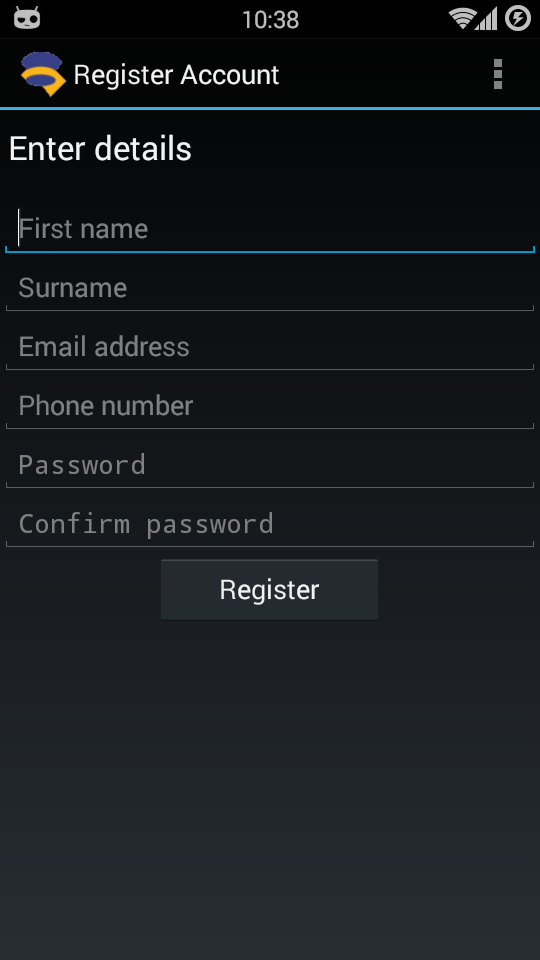
\includegraphics[scale=0.4]{Main App - Registration.png}
\caption{KinderFinder Mobile Application}
\end{figure}

\subsection{Link Restaurant}
After a successful log on, users will have to specify which establishment they are visiting by choosing the restaurant they want to link to. This is done by searching through a list of restaurants using KinderFinder and choosing the one that matches the name of the restaurant the user is dining at.
\begin{figure}[H]
\centering
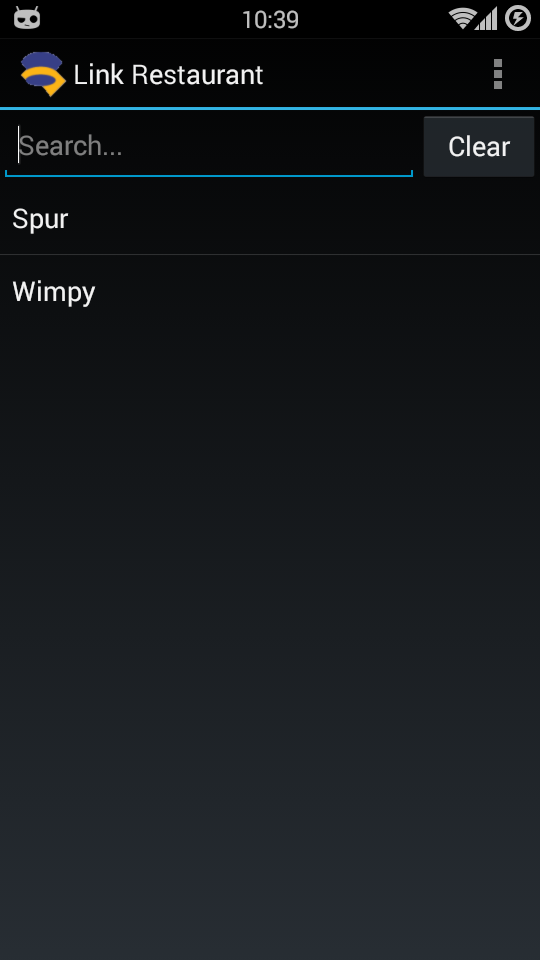
\includegraphics[scale=0.4]{Main App - Link Restaurant.png}
\caption{KinderFinder Mobile Application}
\end{figure}

\subsection{Tags View}
A list of tags registered to the user is shown here, from here one can assign names to tags (to specify and help remember which tag is being worn by a specific child).
\begin{figure}[H]
\centering
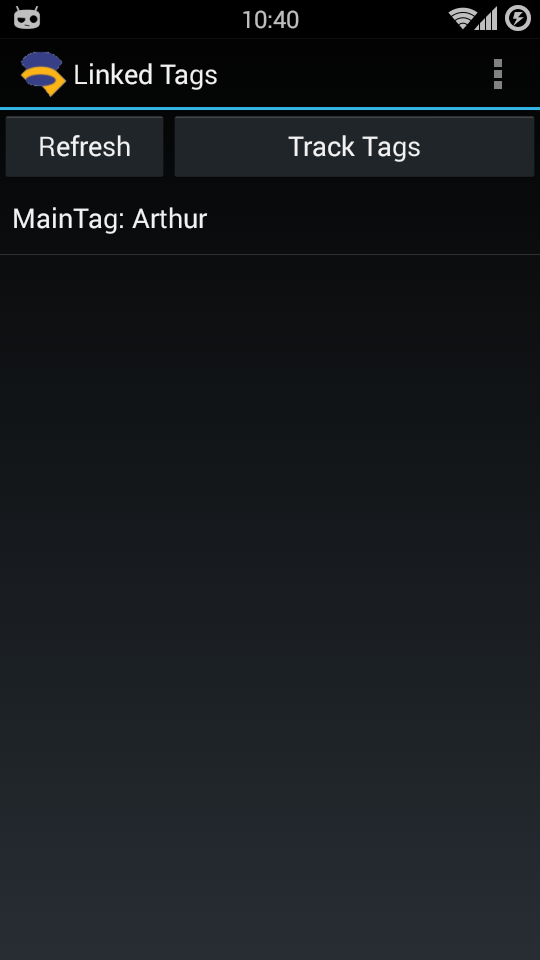
\includegraphics[scale=0.4]{Main App - View Tags.png}
\caption{KinderFinder Mobile Application}
\end{figure}

\subsection{Map view and tracking}
Here, all the tags in the restaurant will be visible on a map of the restaurant areas and zones. If a child goes out of a zone for what ever reason, the phone will vibrate and beep to inform the parent of this.
\begin{figure}[H]
\centering
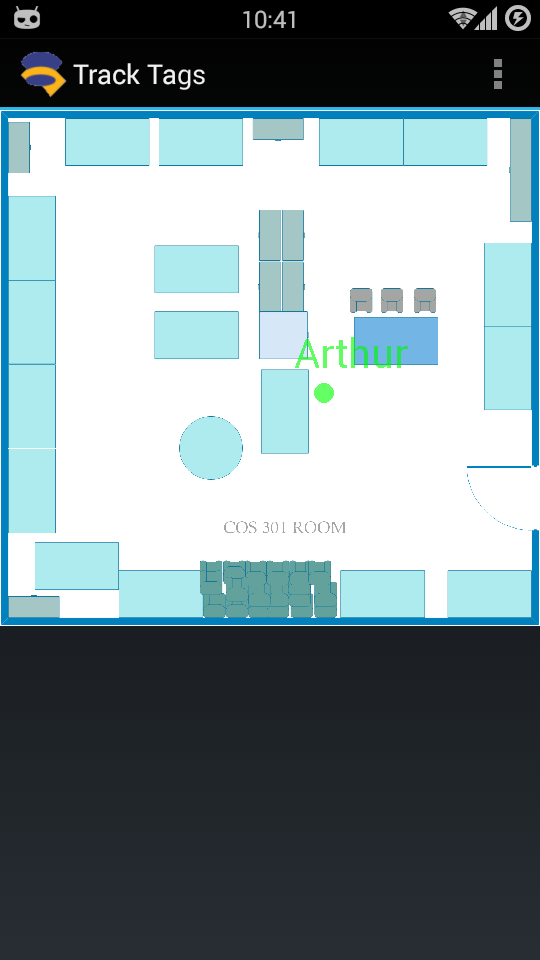
\includegraphics[scale=0.4]{MainAppTrack Tags.png}
\caption{KinderFinder Mobile Application}
\end{figure}









\end{document}
